\documentclass{beamer}
\usetheme{Boadilla}


\graphicspath{ {pic/} }
%for multiline comment
\usepackage{verbatim}

%bibliography
\usepackage{biblatex}
\bibliography{bibliography}

\title{Steiner Triple Systems}
\subtitle{Existence,representation and construction}
\author{Luca Vecchi}
\institute{University of Milan}
\date{\today}

\begin{document}
	%first slide
	\begin{frame}
	\titlepage
	\end{frame}
	
	\begin{frame}
		\frametitle{Outline}
		\begin{itemize}
			\item What is it? 
			\item Challenge on \textit{combinatorial design}:
			\begin{itemize}
				\item existence
				\item representation
				\item construction
			\end{itemize}
		\end{itemize}
	\end{frame}

	%definizione di sts
	%meglio formalismo e da qui si vede il combinatorio e la definizione operativa
	%attenzione che sono insiemi (il codominio è indistinguile (forse))
	
	\begin{frame}
		\frametitle{What is Steiner Triple Systems }
		We are in combinatorial design...
		\begin{block}{Steiner Triple Systems (STS)}
			is an ordered pair $(S,T)$ where $S$ is a finite set of \textit{point}/\textit{symbol} and $T$ is a set of subsets of 3-symbol in which all possible pair of $S$ are contained \textbf{once and only once}.\\
			 
		\end{block}
	
	\pause
	More formally:\\
	\begin{itemize}
		\item define $S$ such that $|S|=v$
		\item 	then $T = \{ \{a,b,c\} \subseteq S\times S \times S\}$\\
		 such that $\forall a,b \in S \times S\quad \sum_{\{x,y,z\} \in T} (\mathbb{I}_{ \{ a,b \} \in \{ (x,y), (x,z) , (y,z)  \} }) = 1 $
	\end{itemize}
	More compact way to define STS by define the \textit{order} $v$ of STS by $v = |S|$
	\end{frame}

\begin{comment}

	\begin{frame}
	\frametitle{Using Columns}
	\begin{columns}
		\column{0.5\textwidth}
		<text>
		\column{0.5\textwidth}
		<text>
	\end{columns}

\begin{description}
	\item[API] Application Programming Interface
	\item[LAN] Local Area Network
	\item[ASCII] American Standard Code for Information Interchange
\end{description}

\begin{table}
	\begin{tabular}{l | c | c | c | c }
		Competitor Name & Swim & Cycle & Run & Total \\
		\hline \hline
		John T & 13:04 & 24:15 & 18:34 & 55:53 \\ 
		Norman P & 8:00 & 22:45 & 23:02 & 53:47\\
		Alex K & 14:00 & 28:00 & n/a & n/a\\
		Sarah H & 9:22 & 21:10 & 24:03 & 54:35 
	\end{tabular}
	\caption{Triathlon results}
\end{table}
	\end{frame}

	\begin{frame}
	\frametitle{Pictures}
	\begin{figure}
		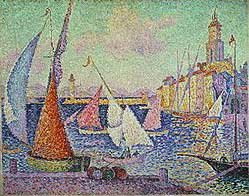
\includegraphics[scale=0.5]{lion}
		\caption{lion!!}
	\end{figure}
	<text>
	\end{frame}
	
	\end{comment}
	
	\begin{frame}
		\frametitle{Bibliography}
		\printbibliography
	\end{frame}
\end{document}